%!TEX root = ../../dokumentation.tex

Both \textit{RabbitMQ} and Apache \textit{Kafka} (hereinafter \enquote{Kafka}) use the same initial setup for prototyping, as shown in Figure \ref{img:prototypeasynccomm}.
The task is to create a topic where ten consumer are subscribed to and each published message from the producer is send to each consumer.
A total of 10000 messages will be sent via the implemented solution, and the consumer checks if the order of the messages was correct.
The time for sending and receiving all messages will be measured.
It should be noted that the measured times will only be used to get the gist of the transmission speeds.
\textit{node.js} will be used for implementation because it is well suited for microservice architecture \cite{AnkitKumar.2019} and has already been used in the prototype for synchronous messaging.
Two \textit{node.js} services are created, and automated with \textit{docker} and \textit{docker-compose}.
The \textit{docker-compose} will also contain the messaging infrastructure.

\begin{figure}[h]
	\centering
	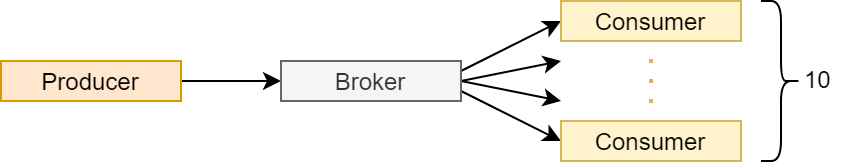
\includegraphics[width=\textwidth, height=0.8\textheight, keepaspectratio]{proto_async.png}
	\caption{Prototype setup for asynchronous communication}
	\label{img:prototypeasynccomm}
\end{figure}

\textbf{RabbitMQ}

The prototypic implementation of \textit{RabbitMQ} will use the \ac{AMQP} protocol as it is the default option.
The consumer and producer services use the \textit{amqplib} library to connect to \textit{RabbitMQ}.
There are other library options, but \textit{amqplib} is the most downloaded one on \textit{npm} \cite{npmtrends.2020}.
\textit{RabbitMQ} also provides an official docker image which was used for this prototype.

The modularity is given since exchanges and queues can be freely defined within the code or via a management interface.
In the prototype, both are created within the code, but this creates coupling between producer and consumer.
The coupling between producer and consumer is shown in Figure \ref{img:rabbitmqproto} by the brackets in the respective color of the producer and consumer.
The producer knows only the exchange definition, while the consumer knows exchange and queue definitions.
It is important to note, that this coupling can be reduced if the exchange and queues are defined via the management interface.

\begin{figure}
	\centering
	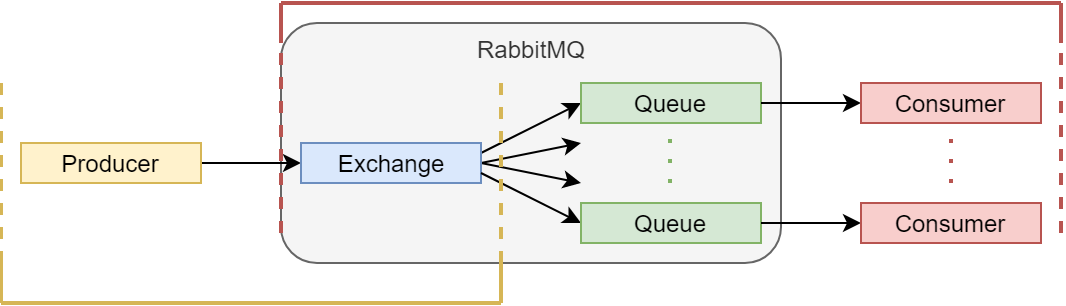
\includegraphics[width=\textwidth, height=0.9\textheight, keepaspectratio]{rabbitmq_proto.png}
	\caption{RabbitMQ prototype implementation}
	\label{img:rabbitmqproto}
\end{figure}

Apart from that, the learning effort for creating the prototype was rather low.
Setting up the \textit{RabbitMQ} instance was straight forward with the official \textit{docker} image and connecting the producer and consumer to the instance was easy due to the code examples from \textit{amqplib}.
However, a lot of repetitive code is required when a consumer connects to multiple queues.
In this case, it would make sense to create a management component.

As mentioned above, the available documentation of \textit{amqplib} contains code examples \cite{MichaelBridgen.25.04.2018}, as well as an extensive \ac{API} documentation \cite{MichaelBridgen.14.05.2020}.
\textit{RabbitMQ} also has extensive documentation available on there homepage, which also explains the concepts of \ac{AMQP} and more.
Since the standard \ac{AMQP} is used, a standard way to implement the communication is provided.
On the contrary, since it is specified by protocol, the available amount of extensions is rather low.
Of course, \textit{RabbitMQ} provides plugins to support \ac{MQTT} and \ac{STOMP}, but otherwise there is very little available.
For \textit{node.js} its the same, there are only different implementations for the protocol or wrapper projects to provide TypeScript support.

\textbf{Apache Kafka}

The prototypical \textit{Kafka} implementation includes a producer and consumer service that use the library \textit{KafkaJS} to connect with \textit{Kafka}.
\textit{KafkaJS} has gained popularity over the last year and is slowly closing the gap to the most popular library \textit{kafka-node}.
These two library's are the most used once \cite{npmtrends.2020b}.
Initially, the prototype used \textit{kafka-node}, but it did not work as planned.
In addition, there is no official \textit{Kafka} \textit{docker} image,  so a few were tested.
The \textit{docker} image \textit{wurstmeister/kafka} was chosen because it is the most used \textit{Kafka} \textit{docker} image on \textit{www.docker.hub} \cite{DockerInc.05.06.2020} and is well documented.
It is important to note that while using \textit{kafka-node}, the \textit{Kafka} image was not fully functioning.
Therefore, it is likely that it would work now, after ensuring that the \textit{Kafka} image works as intended.
Finally, for the official \textit{docker} image of \textit{zookeeper} was used.

This now leads to the actual implementation, which is shown in Figure \ref{img:kafkaproto}.
As in the \textit{RabbitMQ} prototype, only one topic was created.
Normally, to enhance the throughput, multiple partitions within one topic would be used, but when using multiple partition, there is no message ordering guarantee.
The ordering of message is guaranteed only within one partition and not within one topic \cite[p.~30]{Kumar.2017}.
The coupling between producer and consumer is much lower compared to \textit{RabbitMQ}.
Both only need to know the topic name.
The figure also shows that each consumer belongs to a separate consumer group.
This is necessary so that each of the ten consumers receives the messages.

\begin{figure}[h]
	\centering
	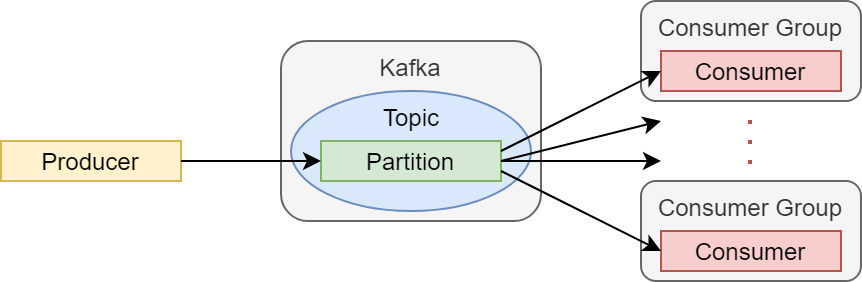
\includegraphics[width=\textwidth, height=0.9\textheight, keepaspectratio]{kafka_proto.png}
	\caption{Apache Kafka prototype implementation}
	\label{img:kafkaproto}
\end{figure}

This results in a higher learning curve than with \textit{RabbitMQ}.
This is mainly because there is no official \textit{Kafka} \textit{docker} image and both the documentation form \textit{wurstmeister/kafka} and \textit{KafkaJS} are extensive and thus it takes time to understand them.
The implementation of the \textit{Kafka} prototype took twice as long as with \textit{RabbitMQ} because the steeper learning curve.
As mentioned above, the documentation available for the used \textit{Kafka} \textit{docker} image and library are extensive.
In case of \textit{KafkaJS}, it contains code examples for getting started as well as a complete description of the producer and consumer functionality and more complex features such as transactions \cite{TulioOrnelas.2020}.
There is also the official \textit{Kafka} documentation to get a more detailed insight about \textit{Kafka} \cite{ApacheKafka.01.06.2020}.
In this prototype, no extensions for \textit{Kafka} were used, but there are some available.
As already explained in \ref{cha:Technologies:communication:kafka}, \textit{Kafka} is the perfect base for an \textit{Event Sourcing} system \cite[p.~19]{Stopford.2018}.
The \textit{AxonFramework} extension aims to extend \textit{Kafka} to provide a framework that can be used to create evolutionary, event-driven microservice systems, based on the principles of Domain Driven Design, Command-Query Responsibility Segregation (CQRS) and Event Sourcing \cite{StevenvanBeelen.29.05.2020}.
Another extension to connect \textit{Kafka} with \textit{Azure} is being created by \textit{Microsoft} \cite{Microsoft.28.05.2020}.
Both extensions are still in the beta phase.
Finally, \textit{Kafka} provides complete freedom in the serialization of data send over or stored within \textit{Kafka}.
The library \textit{Avro} is often used in combination with \textit{Kafka} \cite{JayKreps.2015}.

\textbf{Conclusion}

After implementing a prototype for both asynchronous messaging technologies, the subjective conclusion is that \textit{RabbitMQ} is easier to use.
The main reason are the instructions in the documentation and the provided official \textit{docker} image from \textit{RabbitMQ}.
This made it easy to implement the prototype quickly.
On the other hand, \textit{Kafka}, with its rather complex setup, has a higher skill sealing.
The missing official \textit{docker} image was an issue because every \textit{Kafka} \textit{docker} image must be used sightly different, which leads to search for the right approach.
In the \ac{LAN} application, the required functionality is publish-subscribe to synchronize the microservices.
Therefore, a ordering guarantee and the \ac{QoS} type \textit{at-least-once} are required.

Both Technologies meet the requirements and therefore a benchmark was conducted to evaluate which technology performs better in the given task.
The full benchmark results can be found in the appendix at \ref{chp:appendix:benchmark}.
\textit{RabbitMQ} was significantly faster than \textit{Kafka}.
As a result, \textit{RabbitMQ} was chosen for the \ac{LAN} application because it is faster and easier to use than \textit{Kafka}.
